\section{Our Design}
\label{sec:ourdesign}

After the headroom analysis, we find out that the potential of our dynamic hybrid prefetcher is really encouraging. Here, we come up with our design of dynamic hybrid prefetcher system. We call it \emph{DHP}. The \emph{DHP} is built on the idea of \emph{Static Analysis}. For \emph{Static Analysis}, system takes performace files as input. In \emph{DHP}, these information should be recorded during the execution, using the storage structure explained in section \ref{sec:storestruct}. Then, apply heuristic to these stored information in order to make prefetch decisions.

  \subsection{Storage Structure}
  \label{sec:storestruct}
  \begin{figure}[ht!]
	   \centering
	   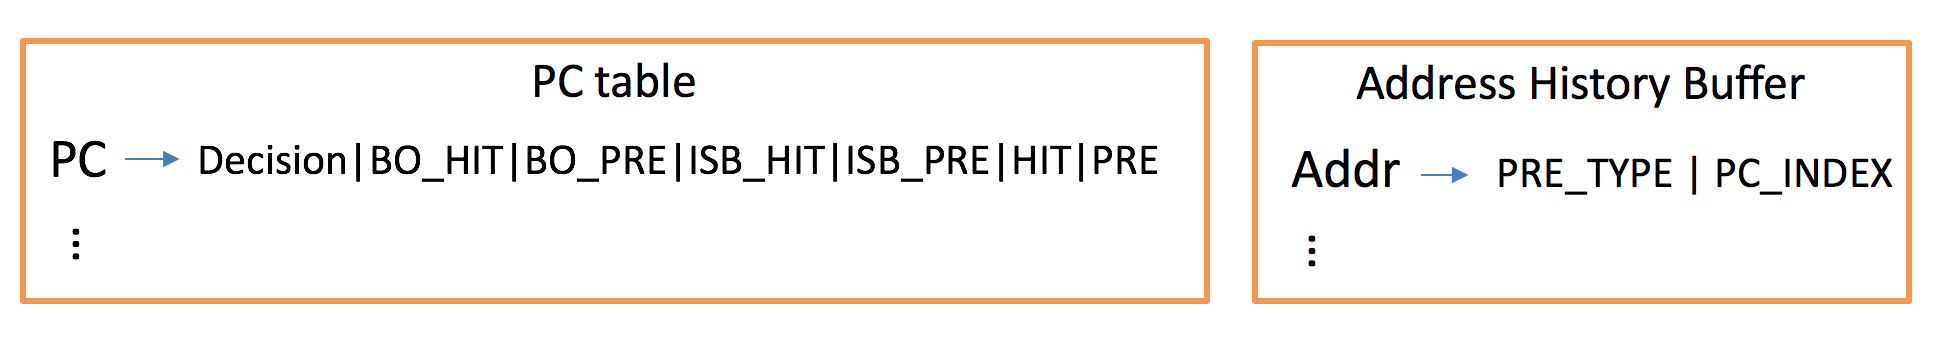
\includegraphics[width=1.0\textwidth]{images/storage_struct.png}
	   \caption{How one PC's and one Addr's information is organized}
	   \label{fig:storage_struct}
  \end{figure}

  The first structure is called \emph{PC Table}. The \emph{PC Table} stores the prefetch information of each prefetcher. Left part of Fig. \ref{fig:storage_struct} shows how one PC's information is stored. \emph{BO/ISB HIT} and \emph{BO/ISB PRE} counts all the prefetches and hits issued by \emph{BO/ISB} using this PC. \emph{HIT} and \emph{PRE} count all the prefetches and hits made by this PC. Last but not least, \emph{Decision} represents the choice of this PC. Usually the number of load PC won't be too large, we choose 4096 as our PC table length.

  On the other hand, if there is a prefetch hit or the cache controller issues a prefetch, the corresponding address needs to know which PC actually prefetched it, so as to increment the correspoinding counter. Here we design the \emph{Address History Table}. \emph{PRE\_TYPE} represents which prefetcher issued the prefetch. It can be \emph{BOTH, ISB} or \emph{BO}. The \emph{PC\_Index} domain stores a back pointer pointing to the corresponding entry of the \emph{PC Table}. Actually one more slot is added to one Addr line, whose name is \emph{DANGER}. Sometimes different PC may prefetch the same address, the \emph{DANGER} value helps decide whether we need to change the PC index entry. Different from PC table, number of addresses visited in one benchmark is far more than the number of PC. Therefore, we design our \emph{Address History Buffer} using 8*4096 entries. Old entries will be replaced if the \emph{Address History Buffer} is full.

  \subsection{Design Overview}
  \label{sec:dynamicdesignoverview}
  \begin{figure}[ht!]
	   \centering
	   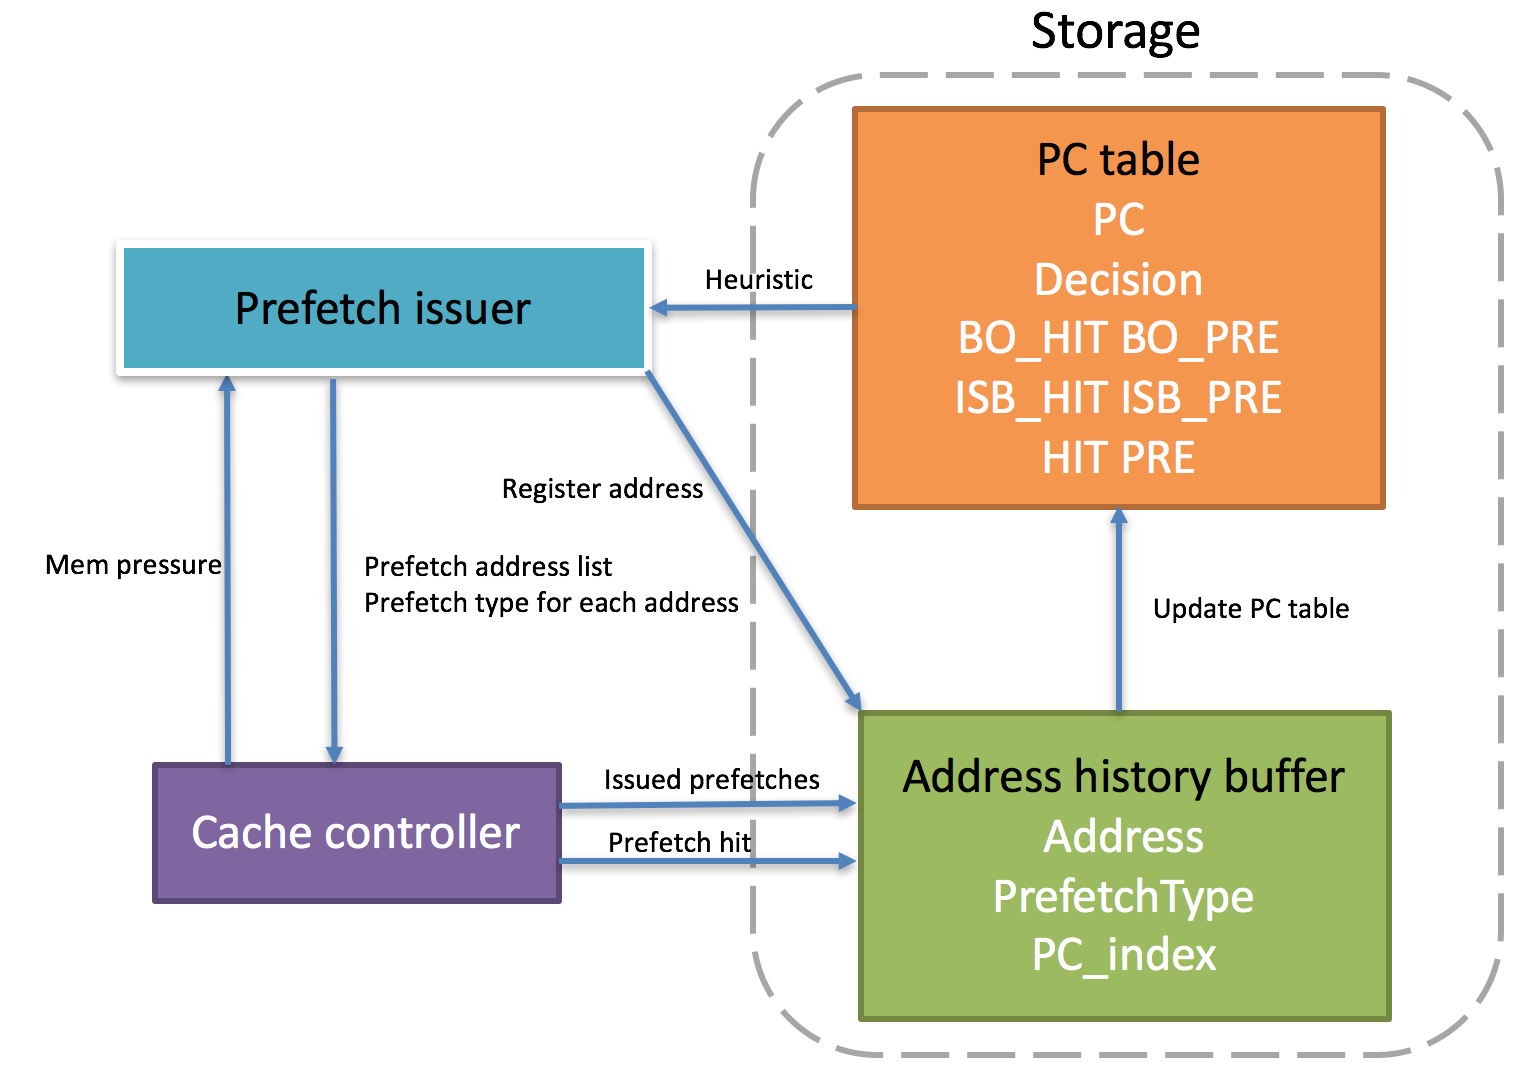
\includegraphics[width=0.8\textwidth]{images/dynamic_design.png}
	   \caption{Headroom speedup under different memory bandwidth}
	   \label{fig:dynamic_design}
  \end{figure}

  In Fig. \ref{fig:dynamic_design}, we show the our design of \emph{DHP}. The \emph{PC Table} and the \emph{Address History Buffer} serves the role of input files in \emph{Static Analysis} case. The update of \emph{PC Table} and \emph{Address History Buffer} is designed asynchronously.

  For the \emph{Address History Buffer}, each time when the \emph{getNextAddress} issues prefetches, it will register the address and its corresponding PC index in the \emph{Address History Buffer}, and initialize this PC if it is not in \emph{PC Table}.

  For \emph{PC Table}'s update, I need to mention two important functions in the file \emph{cache\_cntlr.cc}. One is \emph{doPrefetch} and the other one is \emph{processShmemReqFromPrevCache}. The cache controller receives prefetch list from different prefetcher upon every training. However, it is  \emph{doPrefetch} that actually issues all the prefetching. Each time when \emph{doPrefetch} issues one prefetch, the \emph{Address History Table} will look up this address and update its corresponding PC, same thing happens when a prefetch hit occurs in \emph{processShmemReqFromPrevCache}.

  Each time when one PC's data is updated, heuristics are applid to generate the decision. Obviously the \emph{DHP} need some warm up time for each PC, \emph{DHP} will only issue prefetches both from \emph{ISB} and \emph{BO} when \emph{ISB PRE} is below 1024 and \emph{BO PRE} is below 512.

  In addition, memory usage is also considered in the \emph{DHP}. The memory bus usage or pressure is measured in \emph{cache\_cntlr.cc}. The \emph{DHP} will adjust decision regarding current memory pressure. For example, if the current decision is \emph{BOTH} but the memory bus pressure is high, the \emph{DHP} will only issue the prefetch with higher accuracy. On the other hand, \emph{BOTH} decision are made when the memory bus pressure is low.
